\center{
  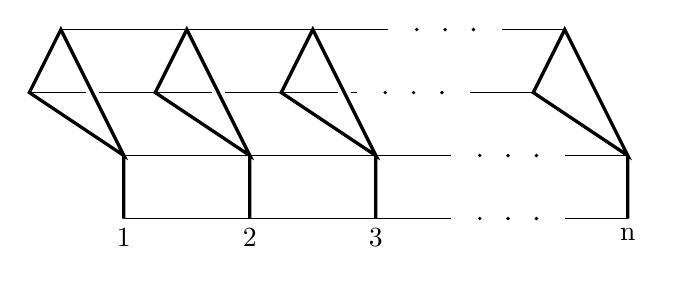
\begin{tikzpicture}[scale=0.8]
    \foreach \x in {0,2,4,8} {
      \draw[very thick] (\x + 2,-1)--(\x + 0.5,0)--(\x + 1,1)--cycle--(\x + 2,-2);
    }
    \draw
      (1,1)--(6.2,1) (8,1)--(9,1)
      (0.5,0)--(1.4,0) (1.6,0)--(3.4,0) (3.6,0)--(5.4,0) (5.6,0)--(5.7,0) (7.5,0)--(8.5,0)
      (2,-1)--(7.2,-1) (9,-1)--(10,-1)
      (2,-2)--(7.2,-2) (9,-2)--(10,-2)
    ;
    \fill
      (6.65, 1) circle (0.03) (7.10, 1) circle (0.03) (7.55, 1) circle (0.03)
      (6.15, 0) circle (0.03) (6.60, 0) circle (0.03) (7.05, 0) circle (0.03)
      (7.65, -1) circle (0.03) (8.10, -1) circle (0.03) (8.55, -1) circle (0.03)
      (7.65, -2) circle (0.03) (8.10, -2) circle (0.03) (8.55, -2) circle (0.03)
    ;
    \node[below] at (2,-2) {1};
    \node[below] at (4,-2) {2};
    \node[below] at (6,-2) {3};
    \node[below] at (10,-2) {n};
  \end{tikzpicture}
}